% !TEX program = xelatex
% In emacs, use this to set default compiler to xelatex:
% M-x TeX-engine-set RET xetex RET

\documentclass[xcolor=table,aspectratio=169]{beamer}

\usepackage{fancyvrb}
\usepackage{array}
\usepackage{booktabs}

\setbeamertemplate{navigation symbols}{}

\usepackage{listings}

\usepackage{graphicx}
\usepackage{hanging}
\usepackage{natbib} %citep and citet
\usepackage{amsmath}
\usepackage{mathtools}

\usepackage{xltxtra}
\setsansfont{Arial}
\setmonofont[Mapping=tex-text]{Arial}

\bibliographystyle{apalike}

\newenvironment{myenumerate}
{\begin{enumerate}
		\setlength{\itemsep}{1pt}
		\setlength{\parskip}{0pt}
		\setlength{\parsep}{0pt}}
	{\end{enumerate}}

\usetheme{Amsterdam2}
\usecolortheme{rose}
%%%%%%%%%%%%%%%%%%%%%%%%%%%%%%%%%%%%%%%%%%%

\usepackage{fancyvrb}
\newcommand{\VerbBar}{|}
\newcommand{\VERB}{\Verb[commandchars=\\\{\}]}
\DefineVerbatimEnvironment{Highlighting}{Verbatim}{commandchars=\\\{\}}
% Add ',fontsize=\small' for more characters per line
\usepackage{framed}
\definecolor{shadecolor}{RGB}{248,248,248}
\newenvironment{Shaded}{\begin{snugshade}}{\end{snugshade}}
\newcommand{\KeywordTok}[1]{\textcolor[rgb]{0.13,0.29,0.53}{\textbf{{#1}}}}
\newcommand{\DataTypeTok}[1]{\textcolor[rgb]{0.13,0.29,0.53}{{#1}}}
\newcommand{\DecValTok}[1]{\textcolor[rgb]{0.00,0.00,0.81}{{#1}}}
\newcommand{\BaseNTok}[1]{\textcolor[rgb]{0.00,0.00,0.81}{{#1}}}
\newcommand{\FloatTok}[1]{\textcolor[rgb]{0.00,0.00,0.81}{{#1}}}
\newcommand{\ConstantTok}[1]{\textcolor[rgb]{0.00,0.00,0.00}{{#1}}}
\newcommand{\CharTok}[1]{\textcolor[rgb]{0.31,0.60,0.02}{{#1}}}
\newcommand{\SpecialCharTok}[1]{\textcolor[rgb]{0.00,0.00,0.00}{{#1}}}
\newcommand{\StringTok}[1]{\textcolor[rgb]{0.31,0.60,0.02}{{#1}}}
\newcommand{\VerbatimStringTok}[1]{\textcolor[rgb]{0.31,0.60,0.02}{{#1}}}
\newcommand{\SpecialStringTok}[1]{\textcolor[rgb]{0.31,0.60,0.02}{{#1}}}
\newcommand{\ImportTok}[1]{{#1}}
\newcommand{\CommentTok}[1]{\textcolor[rgb]{0.56,0.35,0.01}{\textit{{#1}}}}
\newcommand{\DocumentationTok}[1]{\textcolor[rgb]{0.56,0.35,0.01}{\textbf{\textit{{#1}}}}}
\newcommand{\AnnotationTok}[1]{\textcolor[rgb]{0.56,0.35,0.01}{\textbf{\textit{{#1}}}}}
\newcommand{\CommentVarTok}[1]{\textcolor[rgb]{0.56,0.35,0.01}{\textbf{\textit{{#1}}}}}
\newcommand{\OtherTok}[1]{\textcolor[rgb]{0.56,0.35,0.01}{{#1}}}
\newcommand{\FunctionTok}[1]{\textcolor[rgb]{0.00,0.00,0.00}{{#1}}}
\newcommand{\VariableTok}[1]{\textcolor[rgb]{0.00,0.00,0.00}{{#1}}}
\newcommand{\ControlFlowTok}[1]{\textcolor[rgb]{0.13,0.29,0.53}{\textbf{{#1}}}}
\newcommand{\OperatorTok}[1]{\textcolor[rgb]{0.81,0.36,0.00}{\textbf{{#1}}}}
\newcommand{\BuiltInTok}[1]{{#1}}
\newcommand{\ExtensionTok}[1]{{#1}}
\newcommand{\PreprocessorTok}[1]{\textcolor[rgb]{0.56,0.35,0.01}{\textit{{#1}}}}
\newcommand{\AttributeTok}[1]{\textcolor[rgb]{0.77,0.63,0.00}{{#1}}}
\newcommand{\RegionMarkerTok}[1]{{#1}}
\newcommand{\InformationTok}[1]{\textcolor[rgb]{0.56,0.35,0.01}{\textbf{\textit{{#1}}}}}
\newcommand{\WarningTok}[1]{\textcolor[rgb]{0.56,0.35,0.01}{\textbf{\textit{{#1}}}}}
\newcommand{\AlertTok}[1]{\textcolor[rgb]{0.94,0.16,0.16}{{#1}}}
\newcommand{\ErrorTok}[1]{\textcolor[rgb]{0.64,0.00,0.00}{\textbf{{#1}}}}
\newcommand{\NormalTok}[1]{{#1}}

%%%%%%%%%%%%%%%%%%%%%%%%%%%%%%%%%%%%%%%%%%%%%
\usepackage{color}
\definecolor{mygreen}{rgb}{0,0.6,0}
\definecolor{mygray}{rgb}{0.5,0.5,0.5}
\definecolor{mymauve}{rgb}{0.58,0,0.82}

\beamersetuncovermixins{\opaqueness<1>{25}}{\opaqueness<2->{15}}

%%186     206     17      38      #CE1126                    

\title[SLV: EDA]{
	{\LARGE{Supervised Learning and Visualization}:\\\large{Exploratory Data Analysis}}
}
\institute{
	\footnotesize Department of Methodology and Statistics\\
}
\author[Vink | van Kesteren | van der Heijden]{Gerko Vink\\Erik-Jan van Kesteren\\Peter van der Heijden}
\date{
\includegraphics[height=1.5cm]{pics/uu-logo.png}\\
	
	\footnotesize{\emph{Utrecht Applied Data Science}}}


\newcommand{\referto}[1]{\hfill{\scriptsize{\emph{\color{gray}{#1}}}}}

\begin{document}

\begin{frame}
\maketitle
\end{frame}

%\begin{frame}
%  \tableofcontents
%\end{frame}

\section{Introduction}\subsection{}

\begin{frame}{}
  \begin{columns}
    \begin{column}{.5\textwidth}

      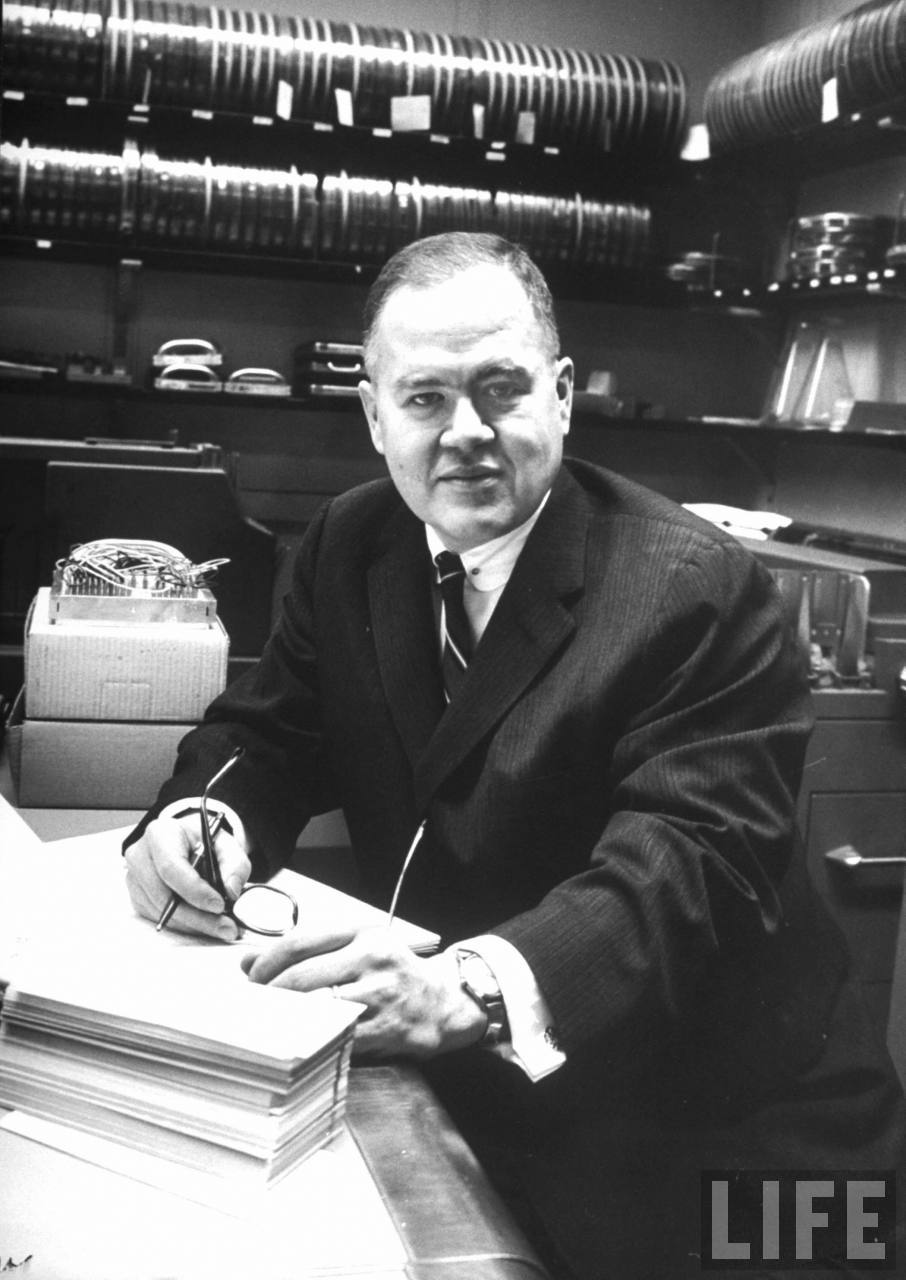
\includegraphics[width=0.78\textwidth]{pics/tukey.jpg}
    \end{column}
    \begin{column}{.5\textwidth}
      \textbf{John Tukey} {\footnotesize (1915--2000)}\\
      \emph{Data Scientist patient zero}\bigskip

      \begin{small}
      Inventor of:
      
      \begin{itemize}
        \item The boxplot
        \item The term ``exploratory data analysis''
        \item The Fast Fourier Transform
        \item ``Tukey's test''
        \item The word ``bit''
        \item So, so much more (Wikipedia)
      \end{itemize}
        
      \end{small}
    \end{column}
  \end{columns}
\end{frame}

\begin{frame}
  Today: visualization principles, applicable to EDA 
\end{frame}
\section{Some visualization principles}\subsection{}

\begin{frame}
  Some data visualization principles
\end{frame}

\begin{frame}
  {Data visualization}

  \begin{itemize}
    \item For exploration, data analysis $\leftarrow$
    \item For communication
    \item For entertainment
  \end{itemize}
\end{frame}

\begin{frame}{}
	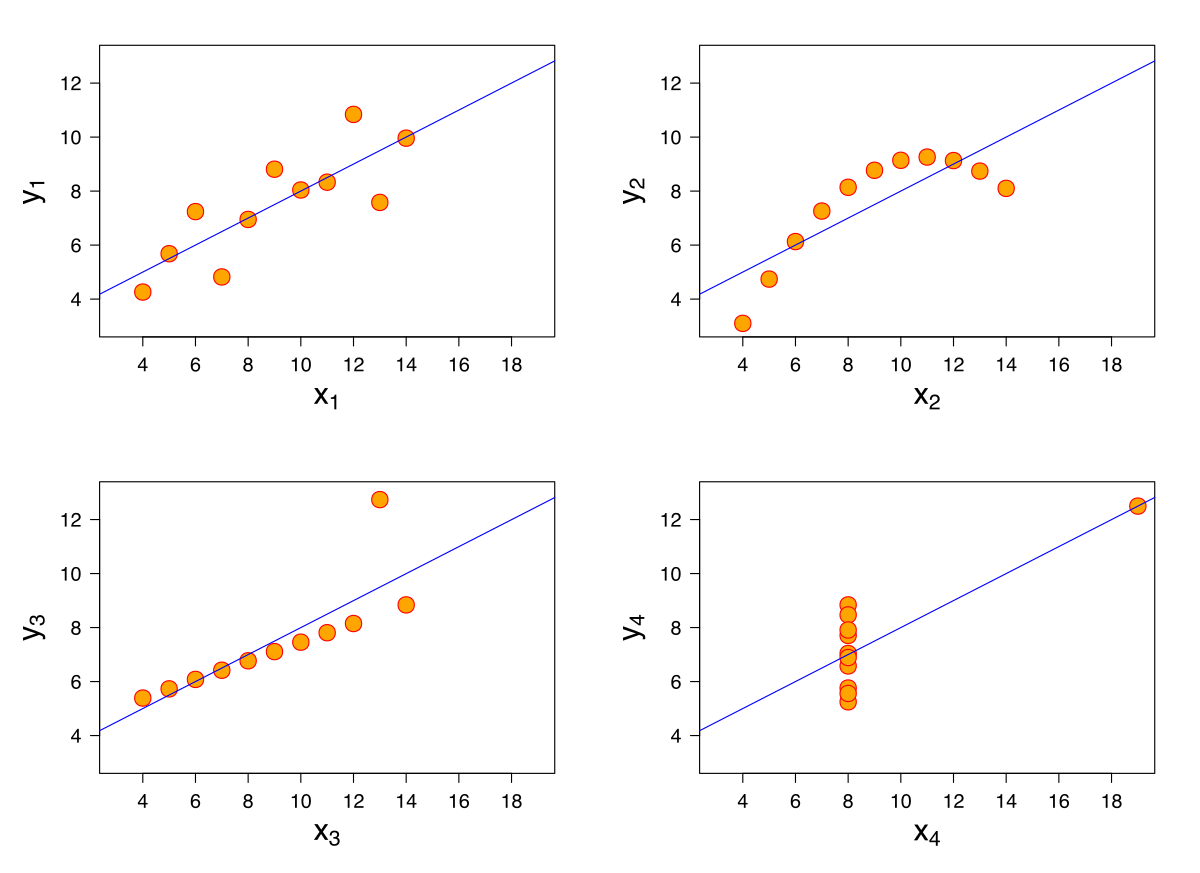
\includegraphics[width=0.78\textwidth]{pics/anscombe.png}
\end{frame}

\begin{frame}{Graphics for data analysis}
  \begin{itemize}
    \item The \textbf{human retina} can transfer around $10^6$ or $10^7$ bits per second to the brain;
    \item \textbf{Reading} transfers about 3 words, so $\sim$ $10^2$ or $10^3$ bits/s;
    \item Potentially (!) visualization is about 4 orders of magnitude more powerful.
      \item[]
      \item[] \textbf{How can we leverage the human visual system to analyze data?}
  \end{itemize}
\end{frame}



\begin{frame}
  {Making pictures that help analyze data}

  \begin{itemize}
  \item We'd like to make, not just any kind of picture or graph, but one that transfers some part of the data to our brain
  \item How do we make sure that the graphs we make transfer
    \begin{enumerate}
    \item The right part of the data, and;
      \item As much of it as possible?
      \end{enumerate}
    \item[]
    \item[] This is where the \textbf{``grammar of graphics''} comes in.
      \item[] Goal is to \textbf{specify how data map to picture}, so the correct type and largest amount possible is transferred
  \end{itemize}
  \end{frame}

\begin{frame}
  {Grammar of graphics (Wickham version)}

  \url{https://r4ds.had.co.nz/data-visualisation.html}
  \bigskip
  
  Map raw data to following elements:
  
  \begin{itemize}
    \item Aesthetics (position, shape, color, ...)
    \item Geometric objects (points, lines, bars, ...)
    \item Scales (continuous, discrete, ...)
    \item Facets (small multiples)
  \end{itemize}

  Additionally, can apply:

  \begin{itemize}
    \item Statistical transformation (identity, binning, median, ...)
    \item Coordinate system (Cartesian, polar, parallel, ...)
  \end{itemize}
\end{frame}
\begin{frame}
  {Grammar of graphics (Wickham version)}

  
  In R, grammar of graphics is implemented in \texttt{ggplot}, a function in the \texttt{ggplot2} package.
  
  
  
\end{frame}

\begin{frame}{Example data set: cars}
  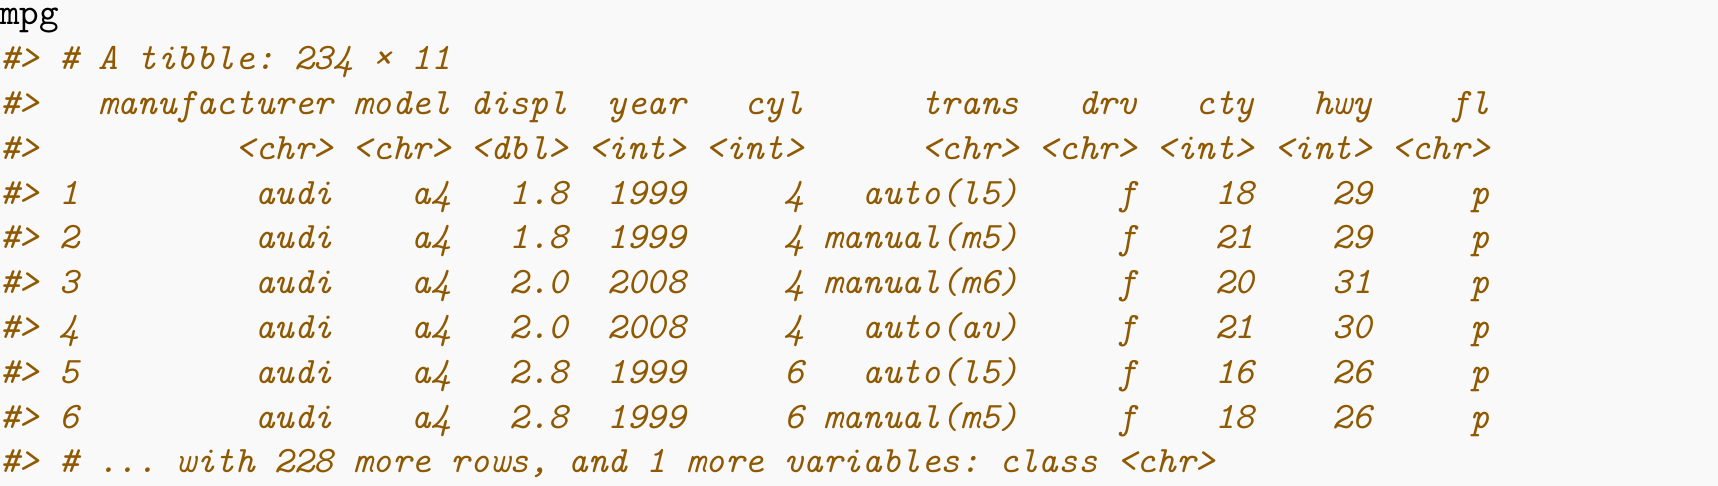
\includegraphics[width=\textwidth]{pics/hadley-cars.png}
\end{frame}

\begin{frame}[fragile]

  \begin{footnotesize}
\begin{verbatim}
ggplot(data = mpg) +
   geom_point(mapping = aes(x = displ, y = hwy, color = class))
\end{verbatim}
  \end{footnotesize}
  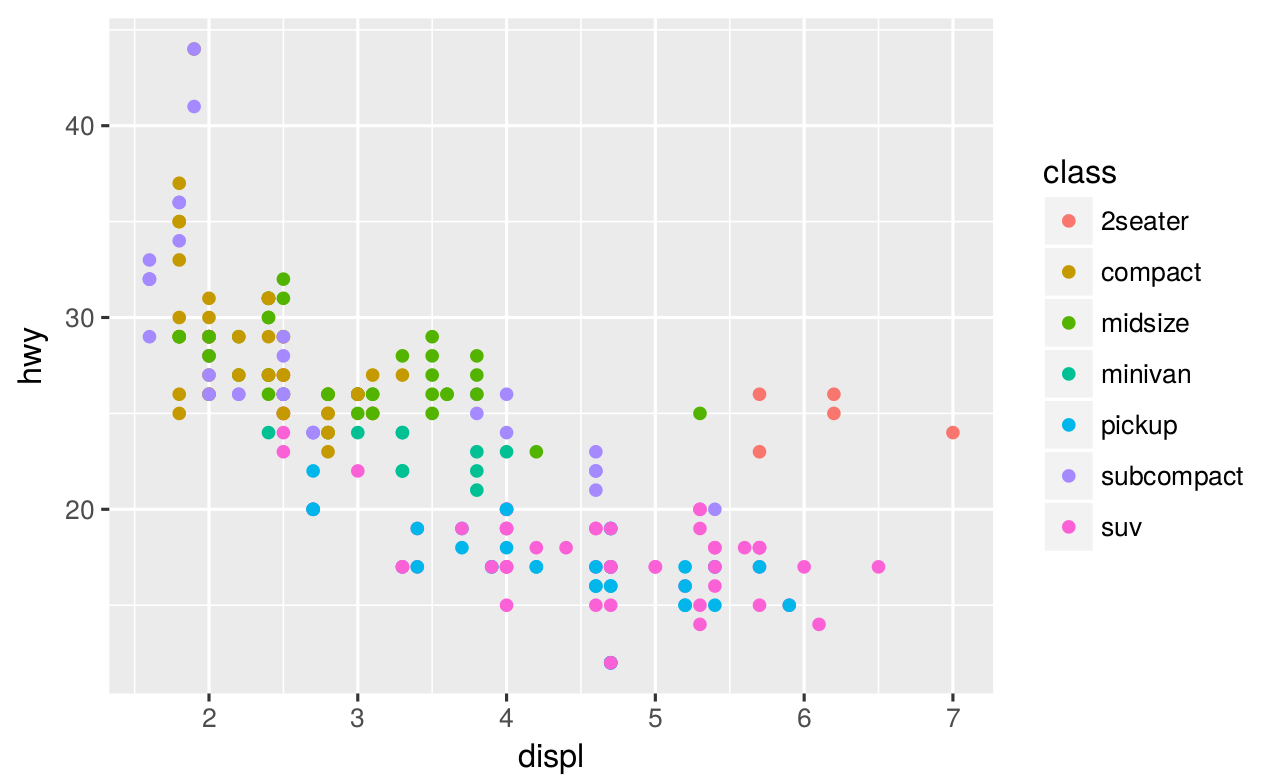
\includegraphics[width=0.78\textwidth]{pics/hadley-simpleplot.png}
\end{frame}

\begin{frame}[fragile]

  \begin{footnotesize}
\begin{verbatim}
ggplot(data = mpg) +
   geom_point(mapping = aes(x = displ, y = hwy, color = class))
\end{verbatim}
  \end{footnotesize}
  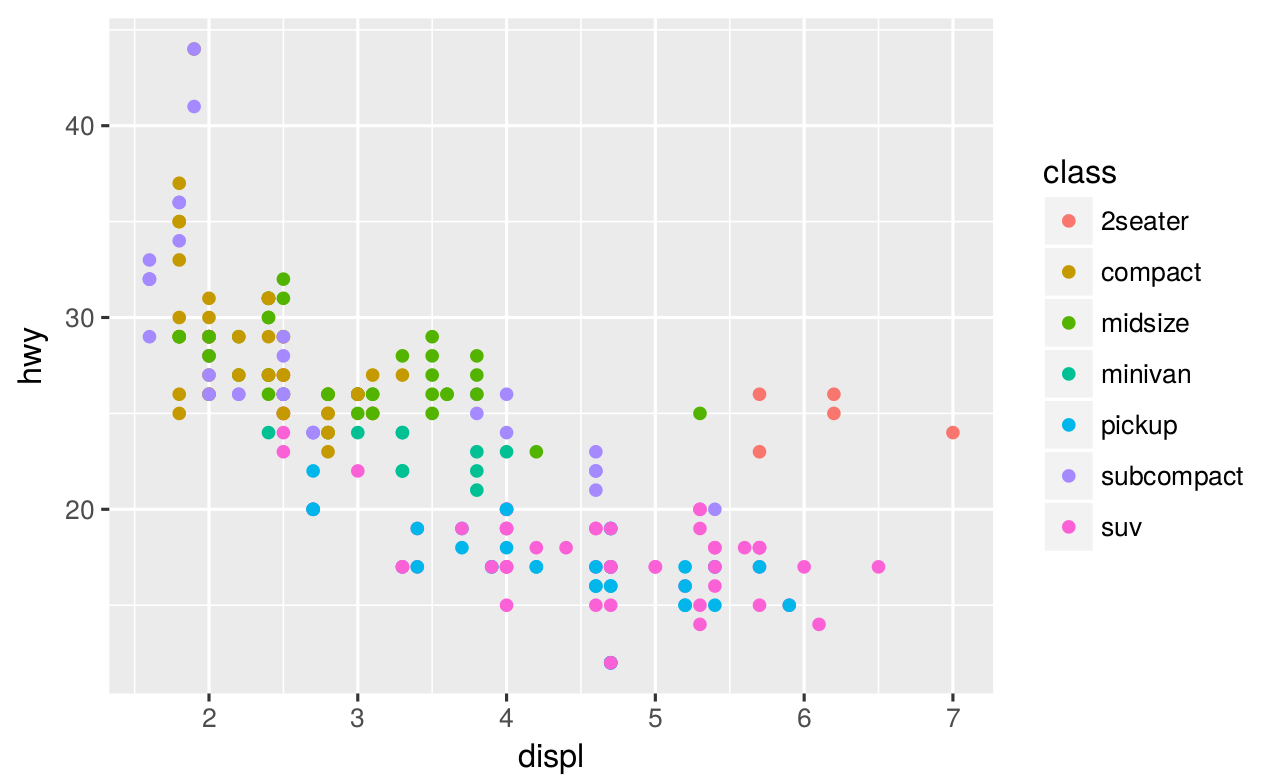
\includegraphics[width=.3\textwidth]{pics/hadley-simpleplot.png}


  \begin{itemize}
  \item Aesthetics:
    \begin{itemize}
    \item     $x$-position mapped to \emph{engine displacement}
    \item   $y$-position mapped to \emph{highway miles per gallon}
      \item color mapped to car type
    \end{itemize}
  \item Geometric objects: points
    \item Transformation: identity 
  \item Scales: continuous, cartesian coordinates
    \item No facets
  \end{itemize}

\end{frame}

\begin{frame}{Facets}
  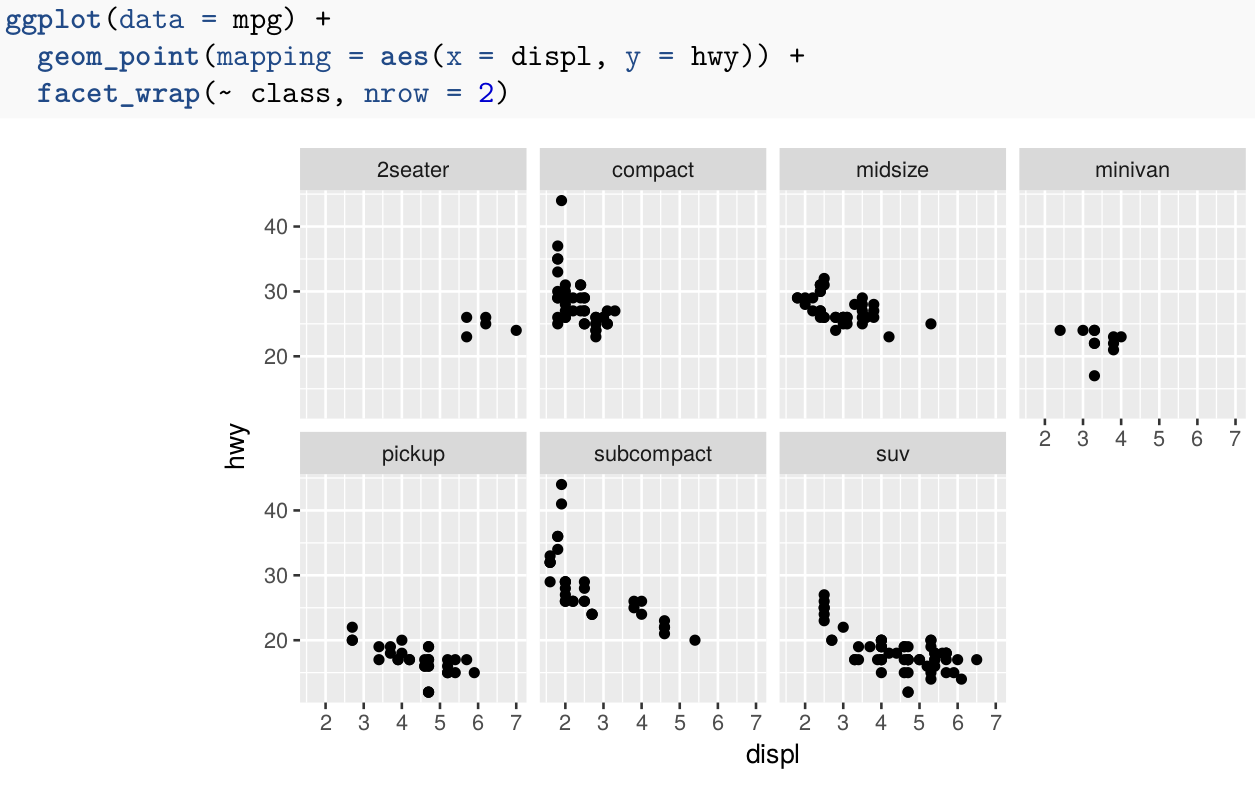
\includegraphics[width=0.78\textwidth]{pics/hadley-facet.png}
\end{frame}

\begin{frame}{Transformation (stats)}
  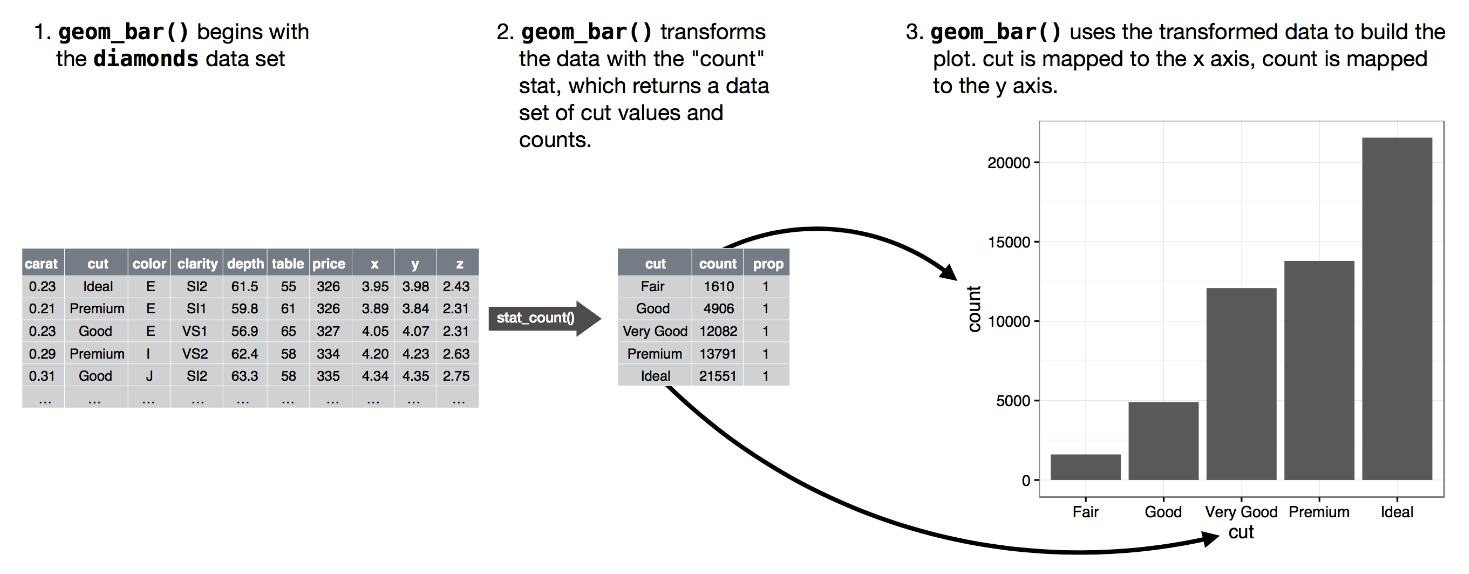
\includegraphics[width=\textwidth]{pics/hadley-stats.png}
\end{frame}

\begin{frame}
  What should I choose?
\end{frame}

\begin{frame}
  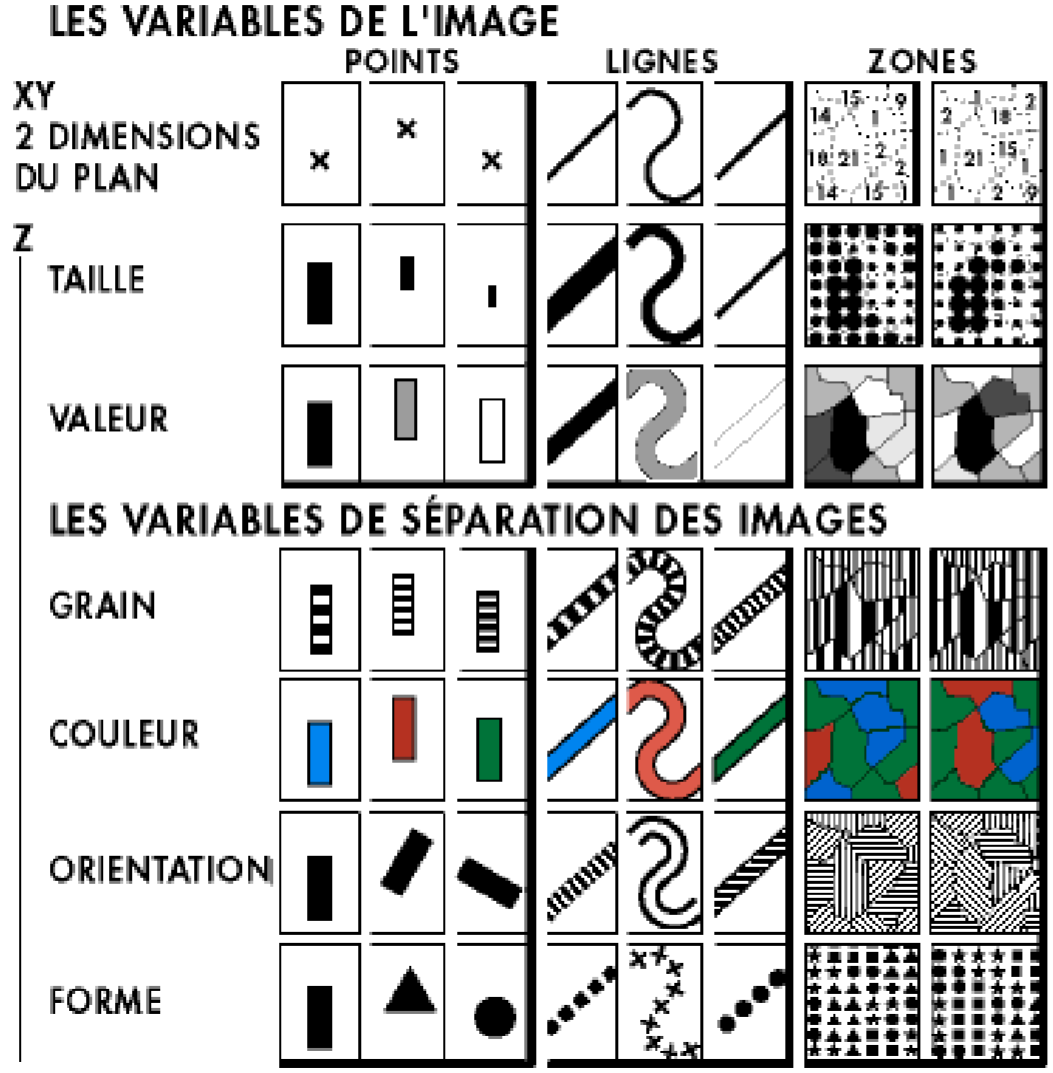
\includegraphics[height=\textheight]{pics/bertin.png} \referto{Jacques Bertin (1967) Sémiologie graphique}
\end{frame}

\begin{frame}{Color: hue-saturation-brightness (HSB)}
  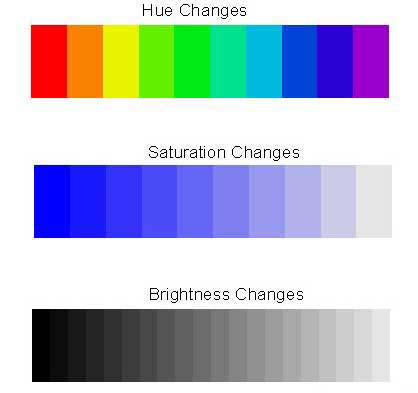
\includegraphics[height=0.8\textheight]{pics/hsb.jpg}
\end{frame}

\begin{frame}{Mackinlay’s ranking of encodings}
  \begin{columns}
    \begin{column}[T]{.3\textwidth}
      \textbf{Quantitative}\medskip

      Position\\
      Length\\
      Angle\\
      Slope\\
      Area\\
      Volume\\
      Density\\
      Color saturation\\
      Color hue\\
      Texture\\
      Connection\\
      Containment\\
      Shape
    \end{column}
    \begin{column}[T]{.3\textwidth}
      \textbf{Ordinal}\medskip
      
      Position\\
      Density\\
      Color saturation\\
      Color hue\\
      Texture\\
      Connection\\
      Containment\\
      Length\\
      Angle\\
      Slope\\
      Area\\
      Volume\\
      Shape
    \end{column}
    \begin{column}[T]{.3\textwidth}
      \textbf{Nominal}\medskip

            Position\\
            Color hue\\
            Texture\\
      Connection\\
      Containment\\         
            Density\\
      Color saturation\\
      Shape\\
      Length\\
      Angle\\
      Slope\\
      Area\\
      Volume

    \end{column}

  \end{columns}
\end{frame}



\begin{frame}
  {Some (distilled) principles from Tufte}

  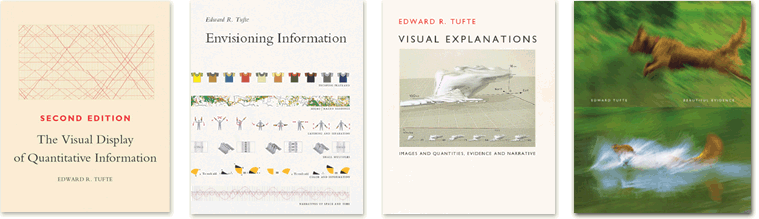
\includegraphics[width=0.8\textwidth]{pics/tufte-bookcovers.png}

  \begin{itemize}

  	\item Ask how data maps to perception
    \item Ask which comparisons you want, guide eye to those
    \item Maximize \textbf{data-to-ink ratio}
    \item Present more data (but without losing interpretability)
    \item (Remember  narrative)
  \end{itemize}
\end{frame}


\begin{frame}
  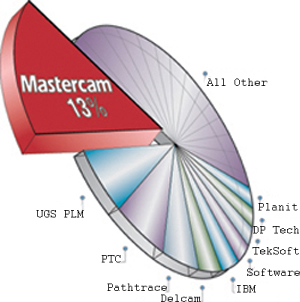
\includegraphics[height=\textheight]{pics/junk.jpg}
\end{frame}



\begin{frame}
  {Nightingale Rose / Coxcomb chart}
  
  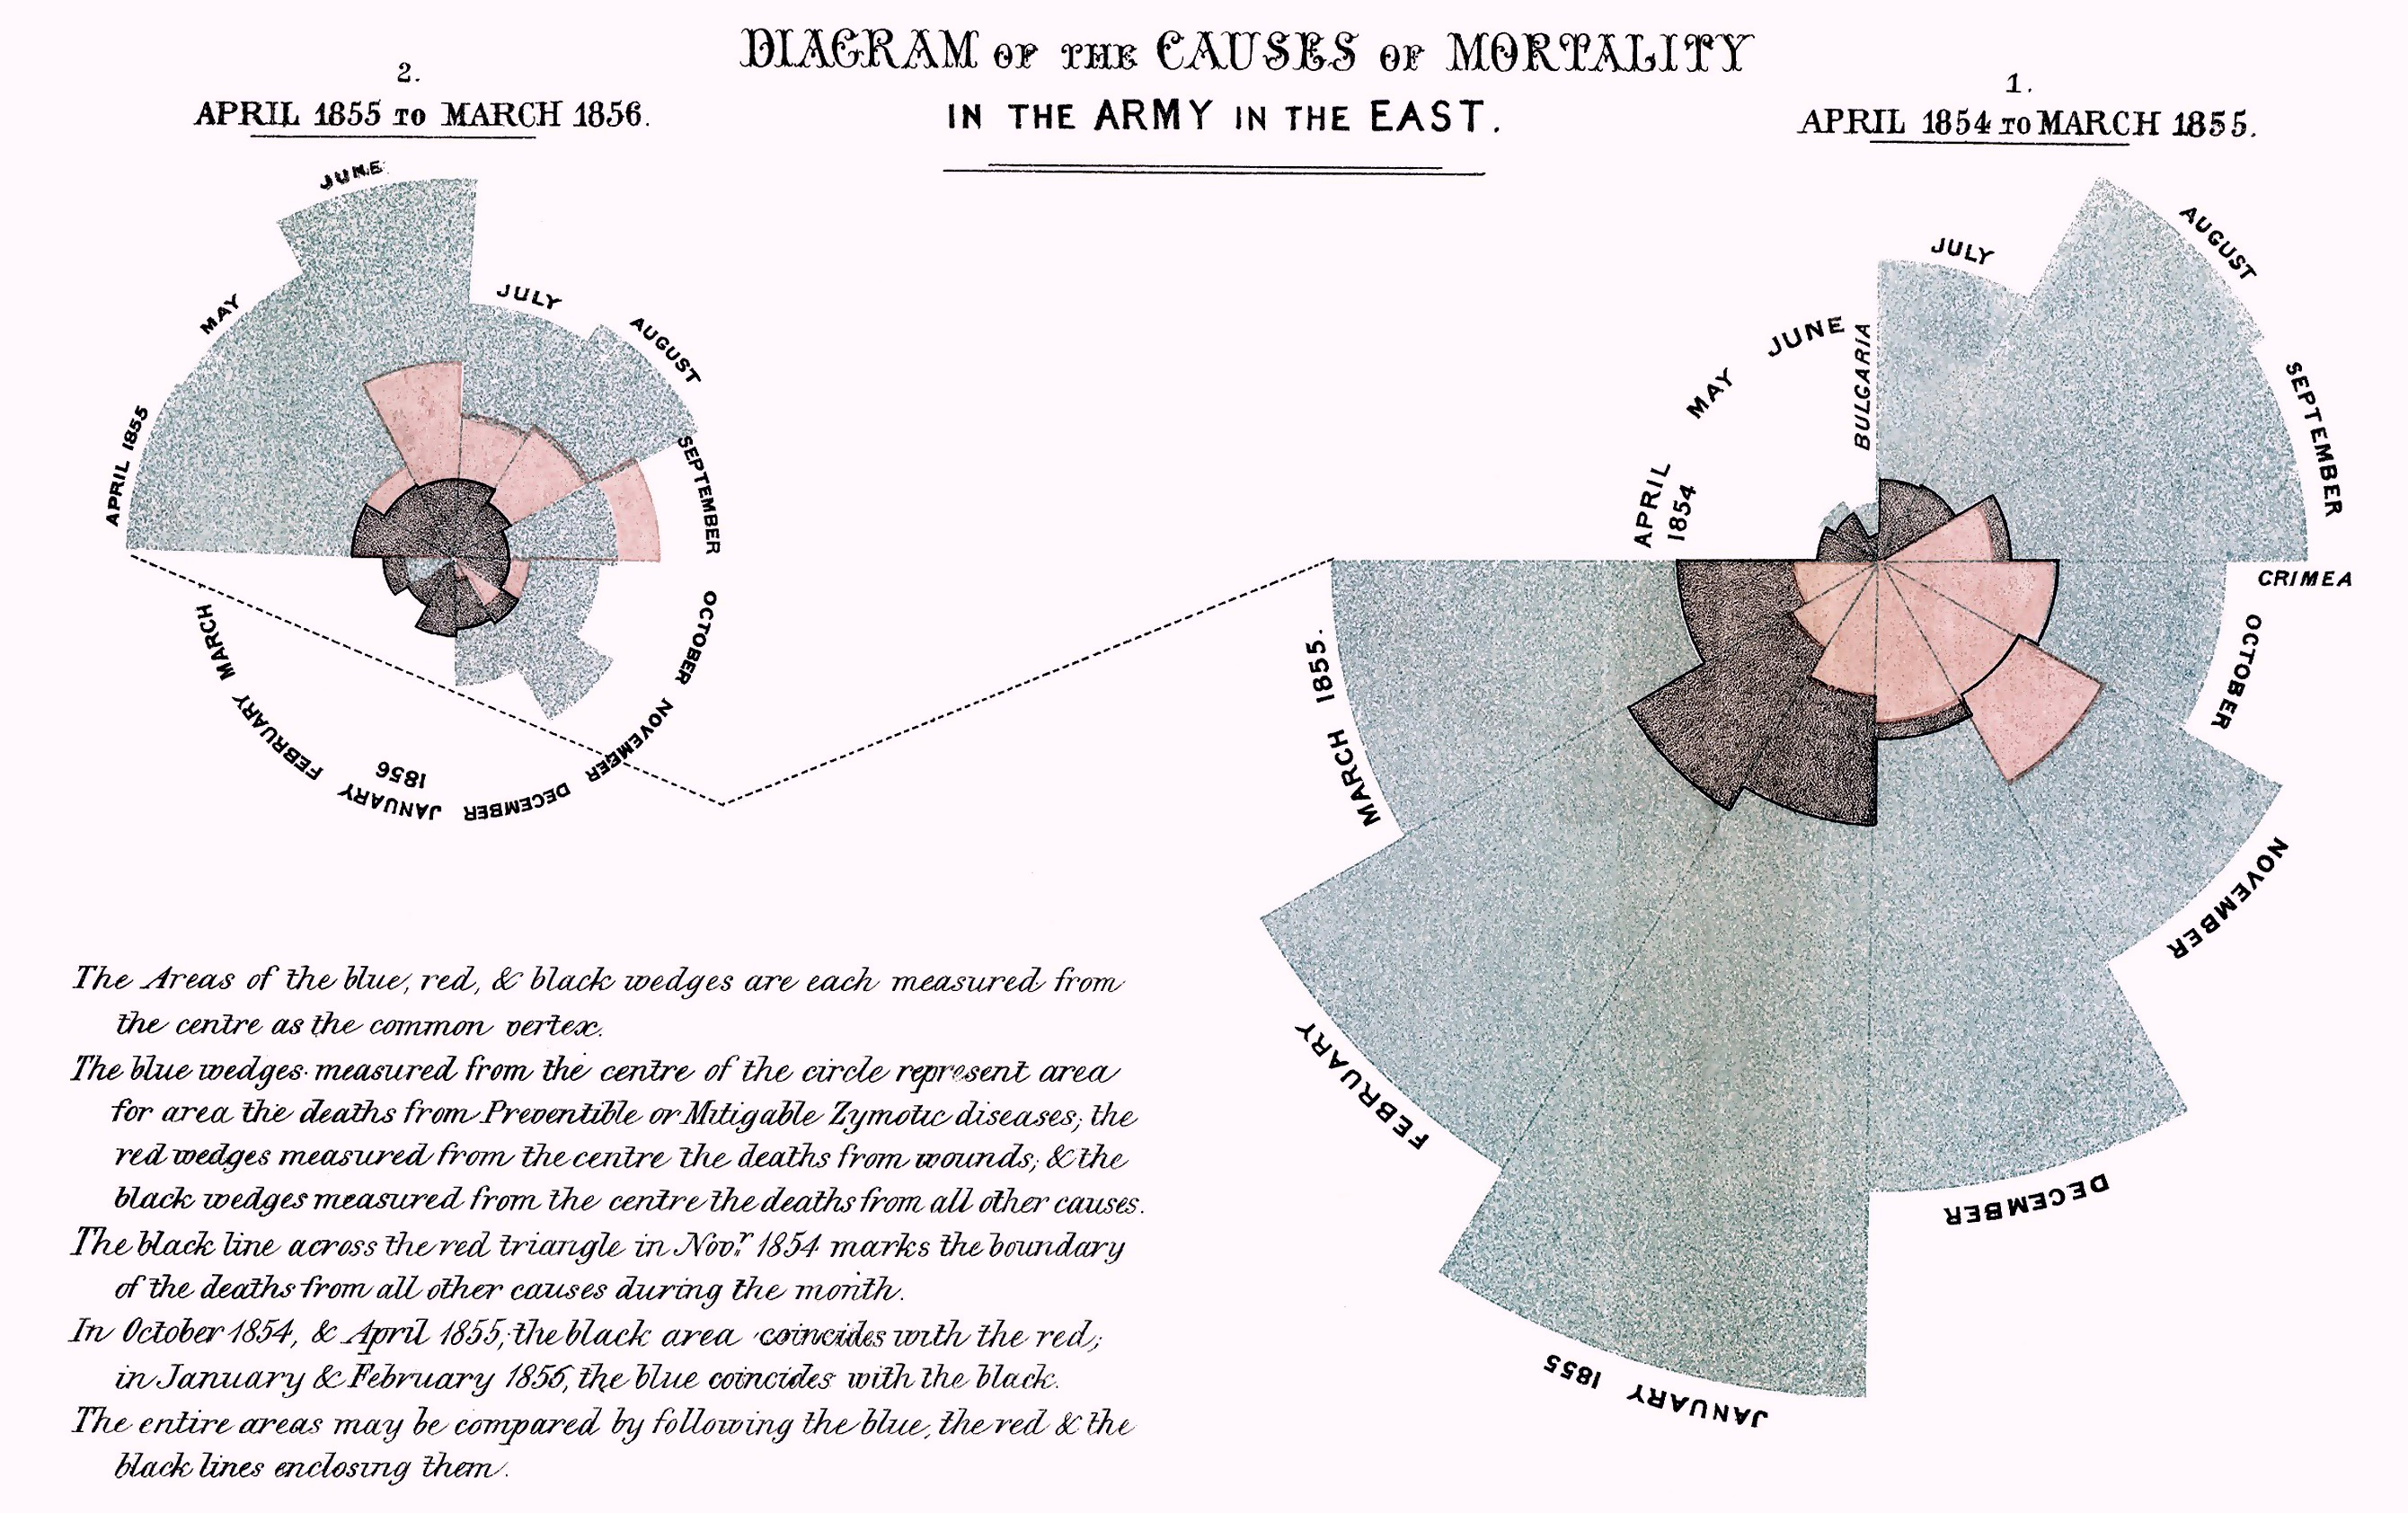
\includegraphics[width=0.8\textwidth]{pics/Nightingale-mortality.jpg}
  
\end{frame}


\begin{frame}
  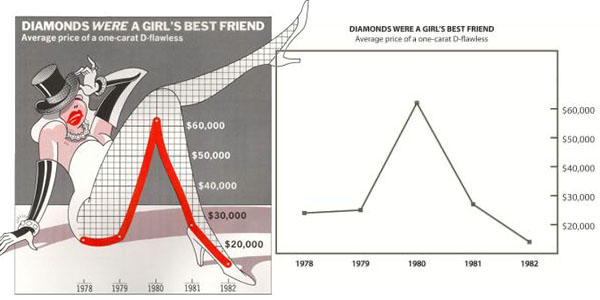
\includegraphics[width=\textwidth]{pics/junk-diamonds.jpg}
\end{frame}

\begin{frame}
	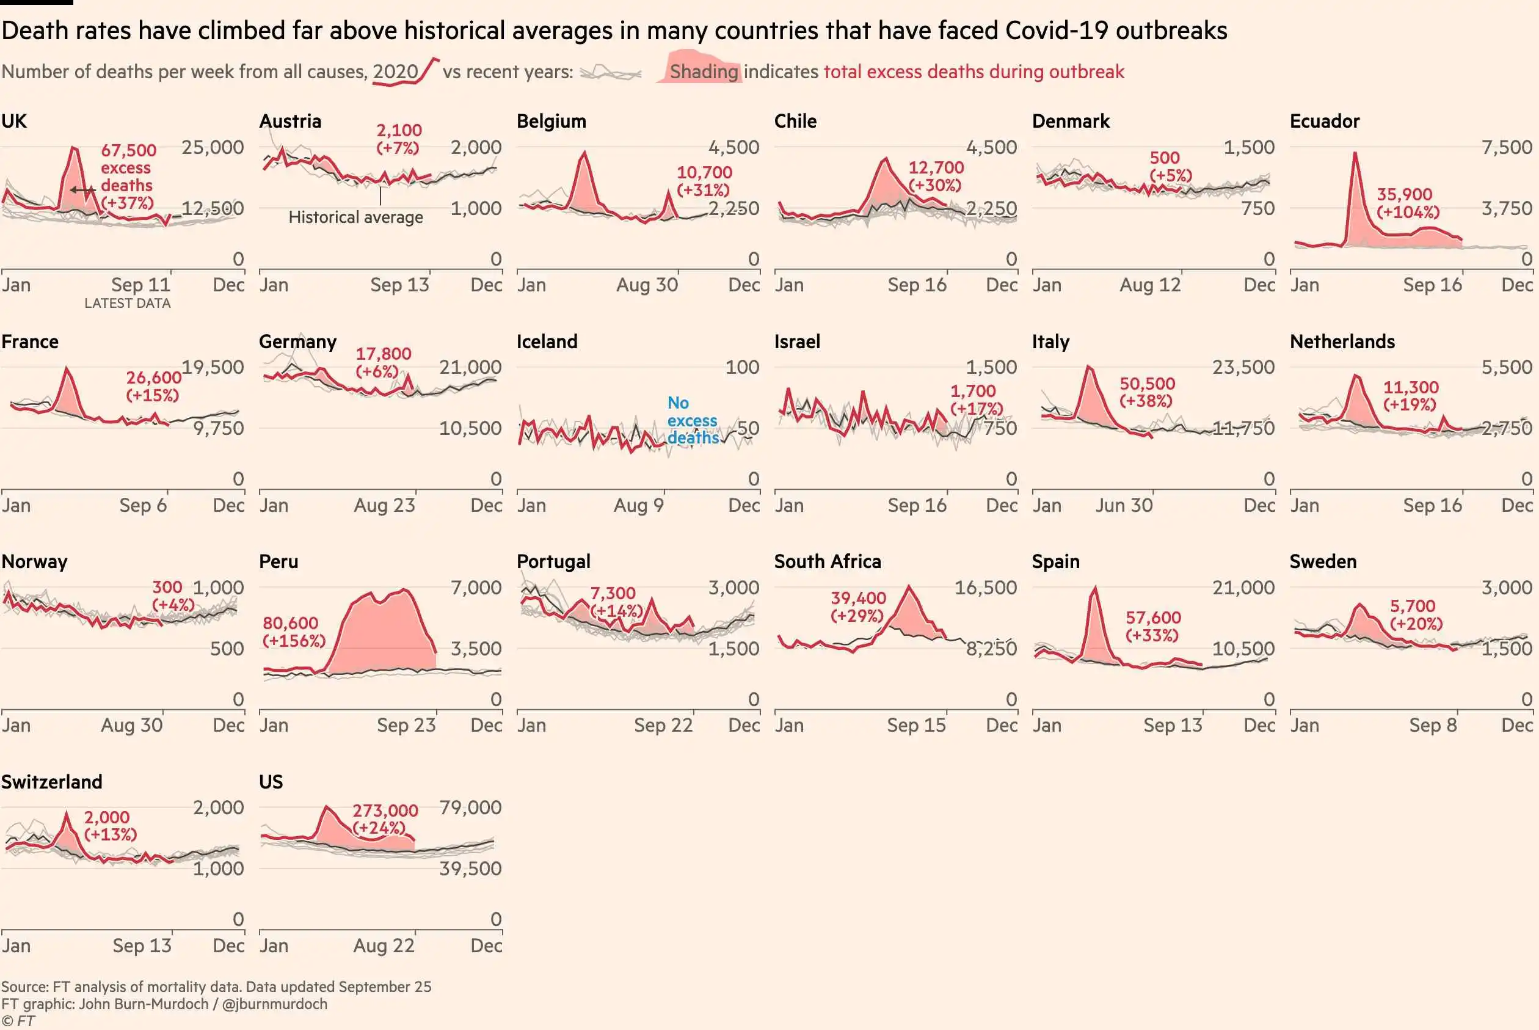
\includegraphics[height=\textheight]{pics/coronavirus_ft.png}
\end{frame}

\begin{frame}
  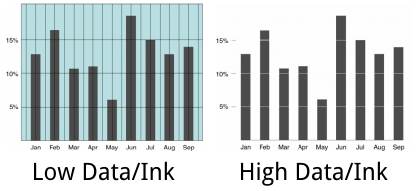
\includegraphics[width=\textwidth]{pics/dataink.png}
\end{frame}

\begin{frame}
  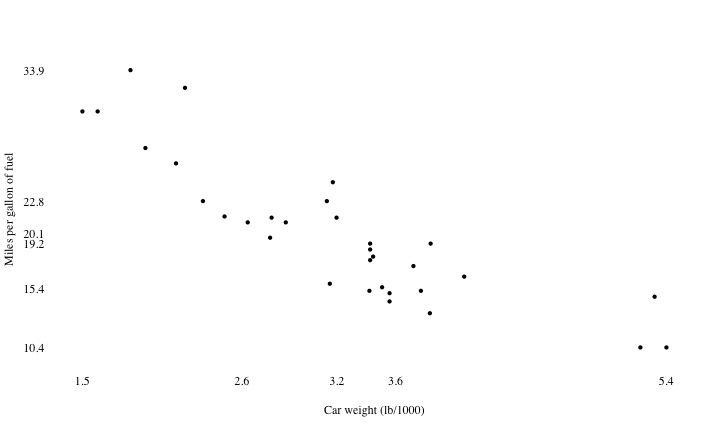
\includegraphics[width=0.78\textwidth]{pics/tufte-scatter.png}
\end{frame}

\begin{frame}
  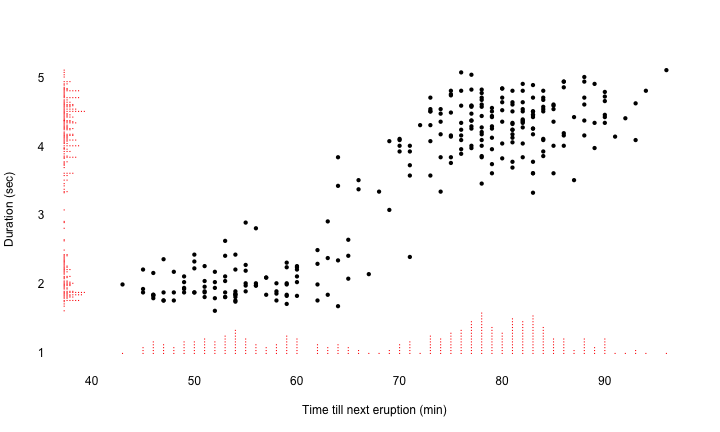
\includegraphics[width=0.78\textwidth]{pics/tufte-scatter2.png}
\end{frame}

\begin{frame}[fragile]
  \begin{footnotesize}
\begin{verbatim}
ggplot(quakes, aes(factor(mag),stations)) + 
   theme_tufte() +
   geom_tufteboxplot(outlier.colour="transparent") + 
   theme(axis.title=element_blank())
\end{verbatim}
  \end{footnotesize}
  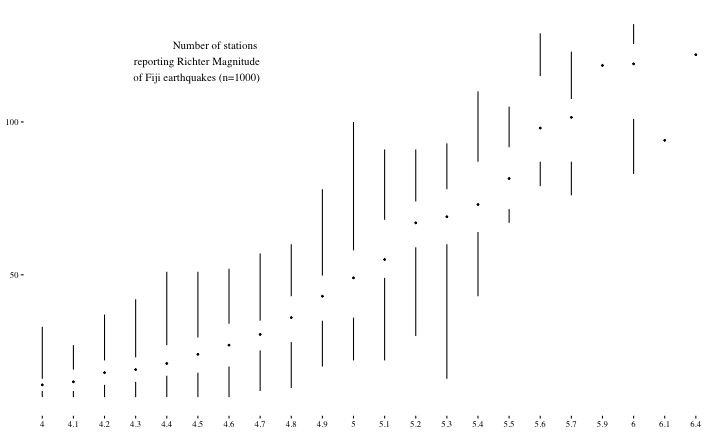
\includegraphics[width=0.68\textwidth]{pics/tufte-box.png}
\end{frame}

\begin{frame}{Tufte wisdom}
  \begin{itemize}
  \item Tufte's principles are more oriented to communication and can be taken too far
    \item[]
  \item Better data/ink $\rightarrow$ display more information without overload;
    \item Thinking about perception can help you choose better geoms, aesthetics. 
    
  \end{itemize}
\end{frame}

\begin{frame}
  Some practice
\end{frame}


\begin{frame}Answer these questions:
  \begin{itemize}
  \item What are: aesthetics, geom, scale, facets, transformation, coordinate system
  \item How is data/ink?
  \item Is perception considered optimally?
   \item Can you think of questions you can't answer from this plot which are in the data?
  \end{itemize}
\end{frame}

\begin{frame}
  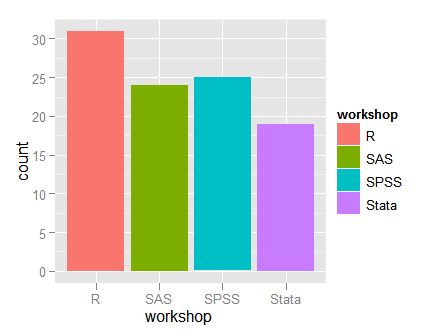
\includegraphics[width=0.7\textwidth]{pics/plot1.png}
\end{frame}


\begin{frame}
  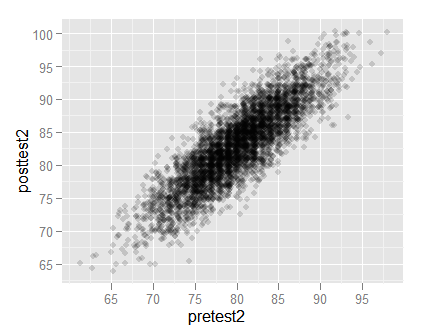
\includegraphics[width=0.7\textwidth]{pics/plot2.png}
\end{frame}


\begin{frame}
  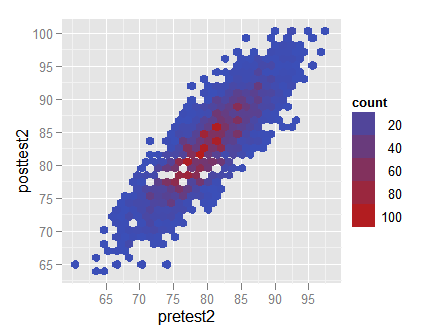
\includegraphics[width=0.7\textwidth]{pics/plot3.png}
\end{frame}

\begin{frame}
  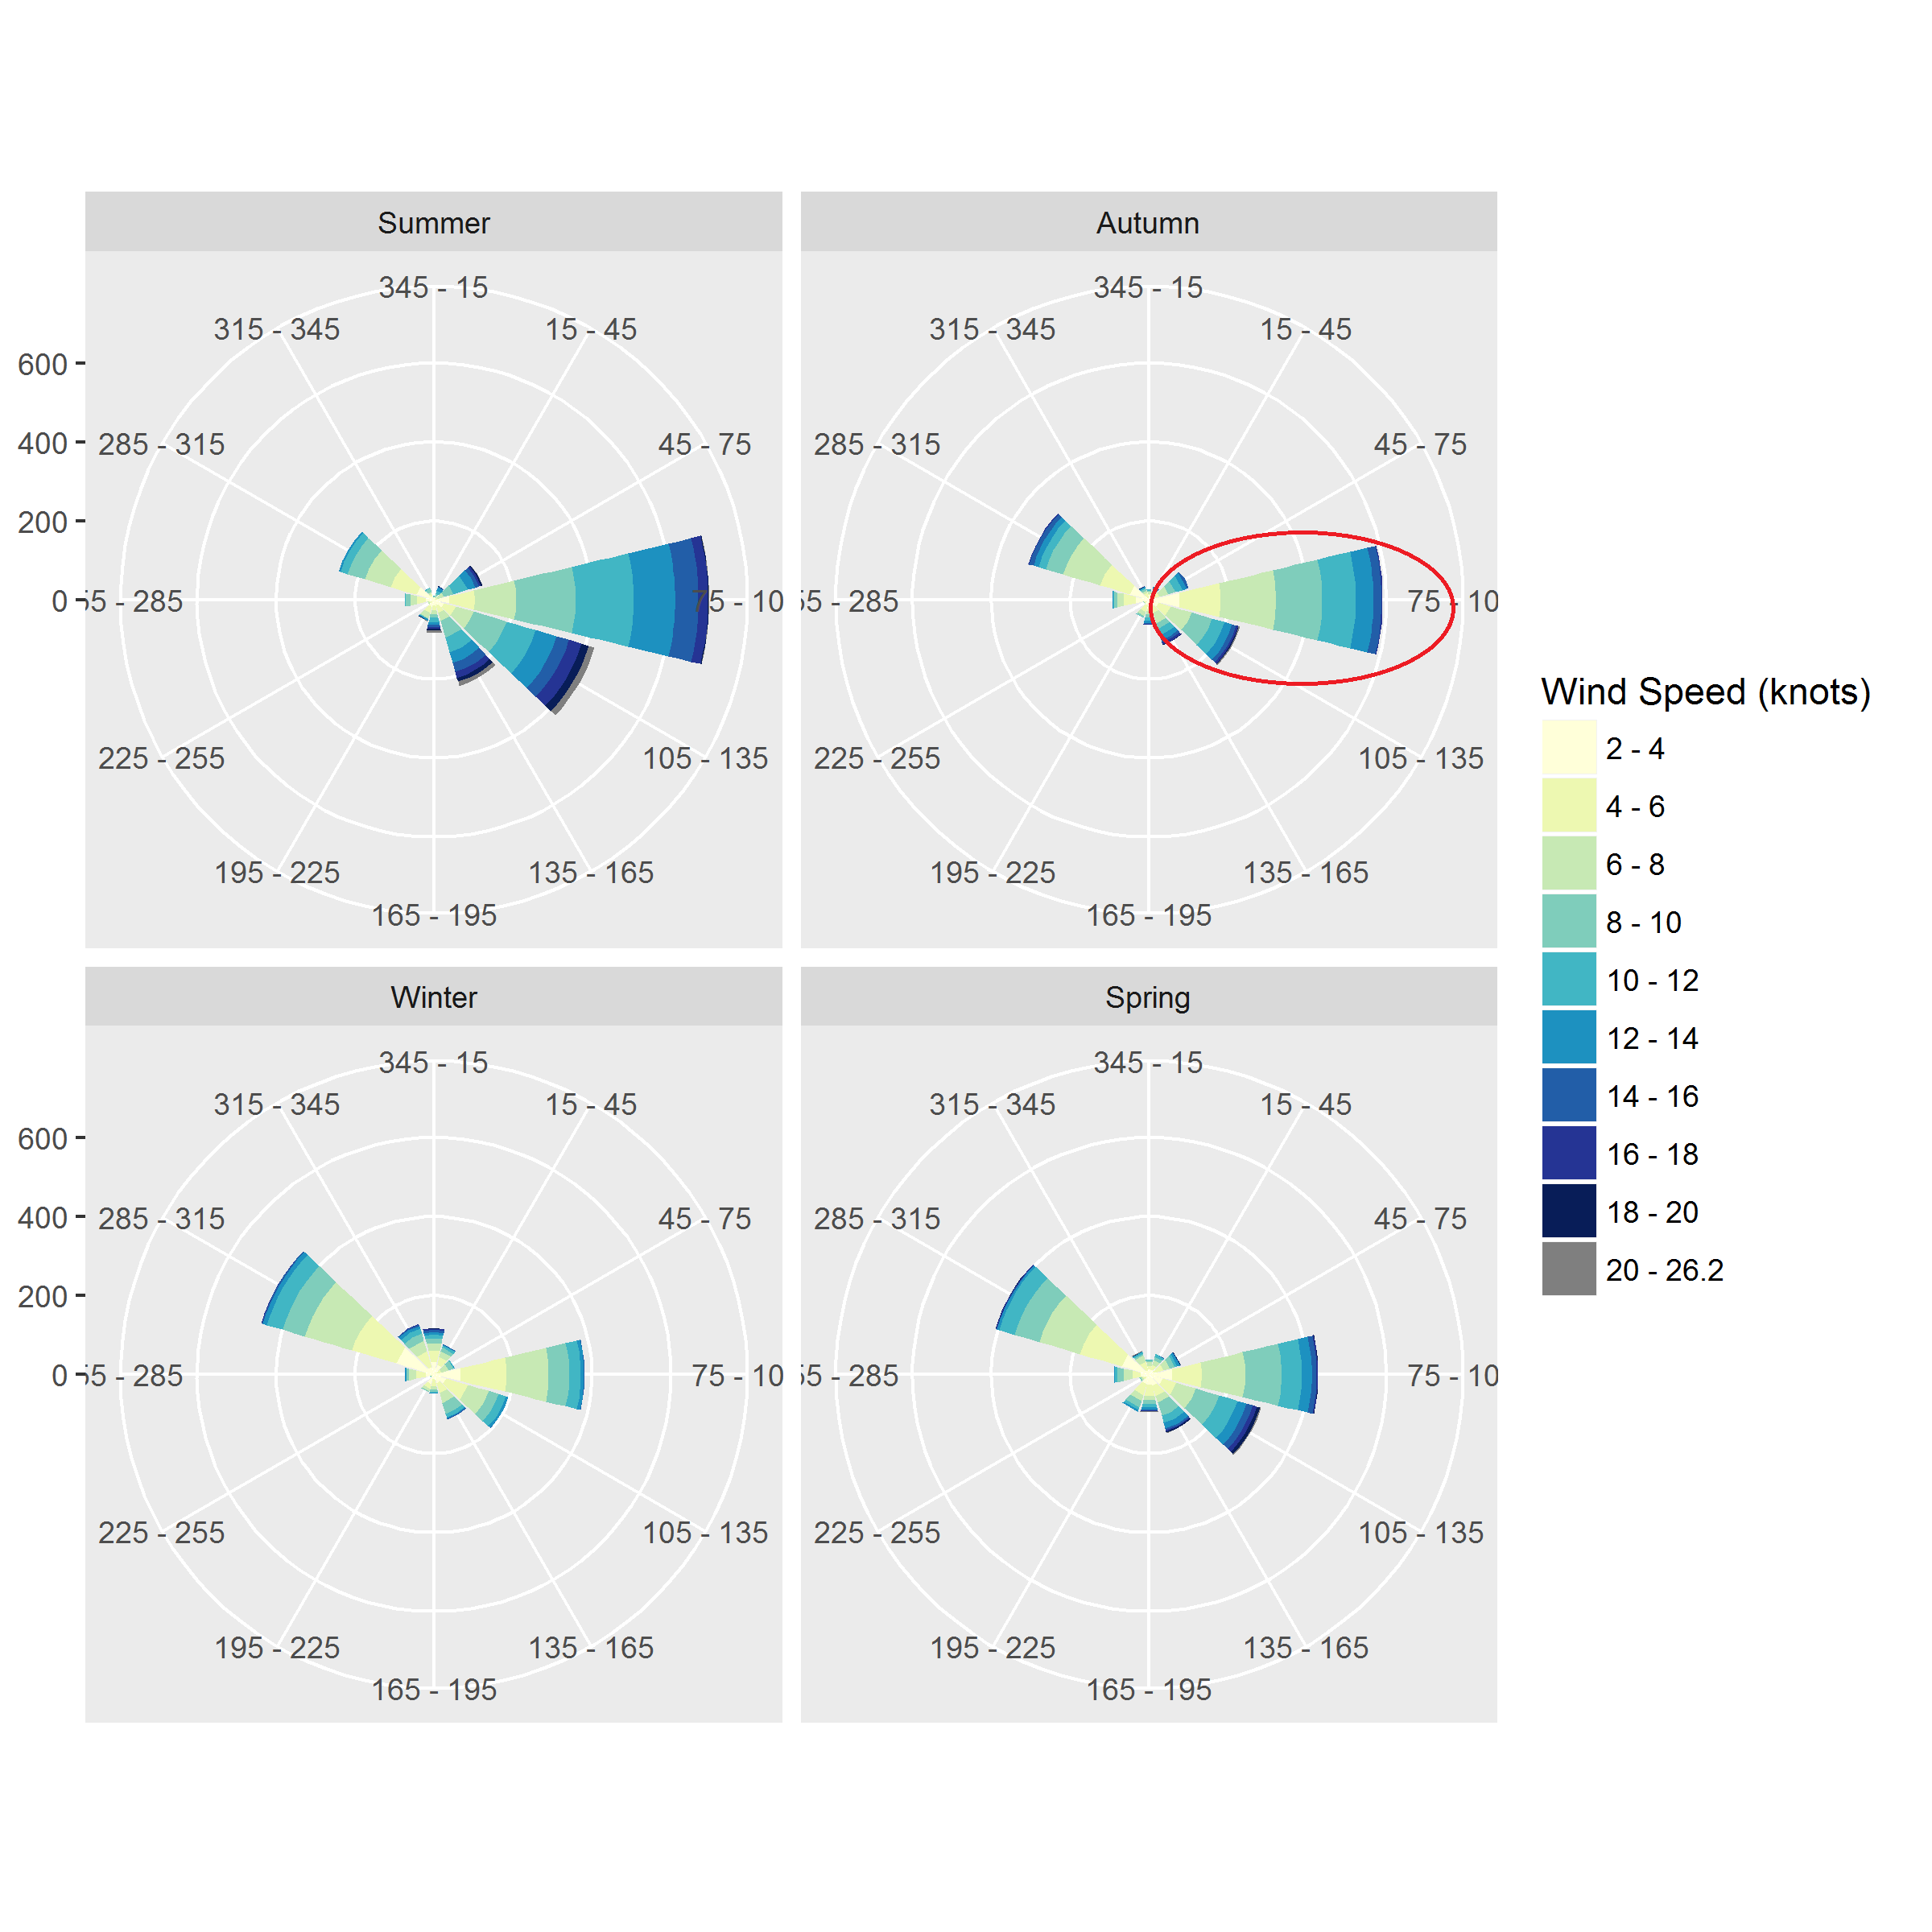
\includegraphics[width=0.6\textwidth]{pics/wind.png}
\end{frame}

\begin{frame}
	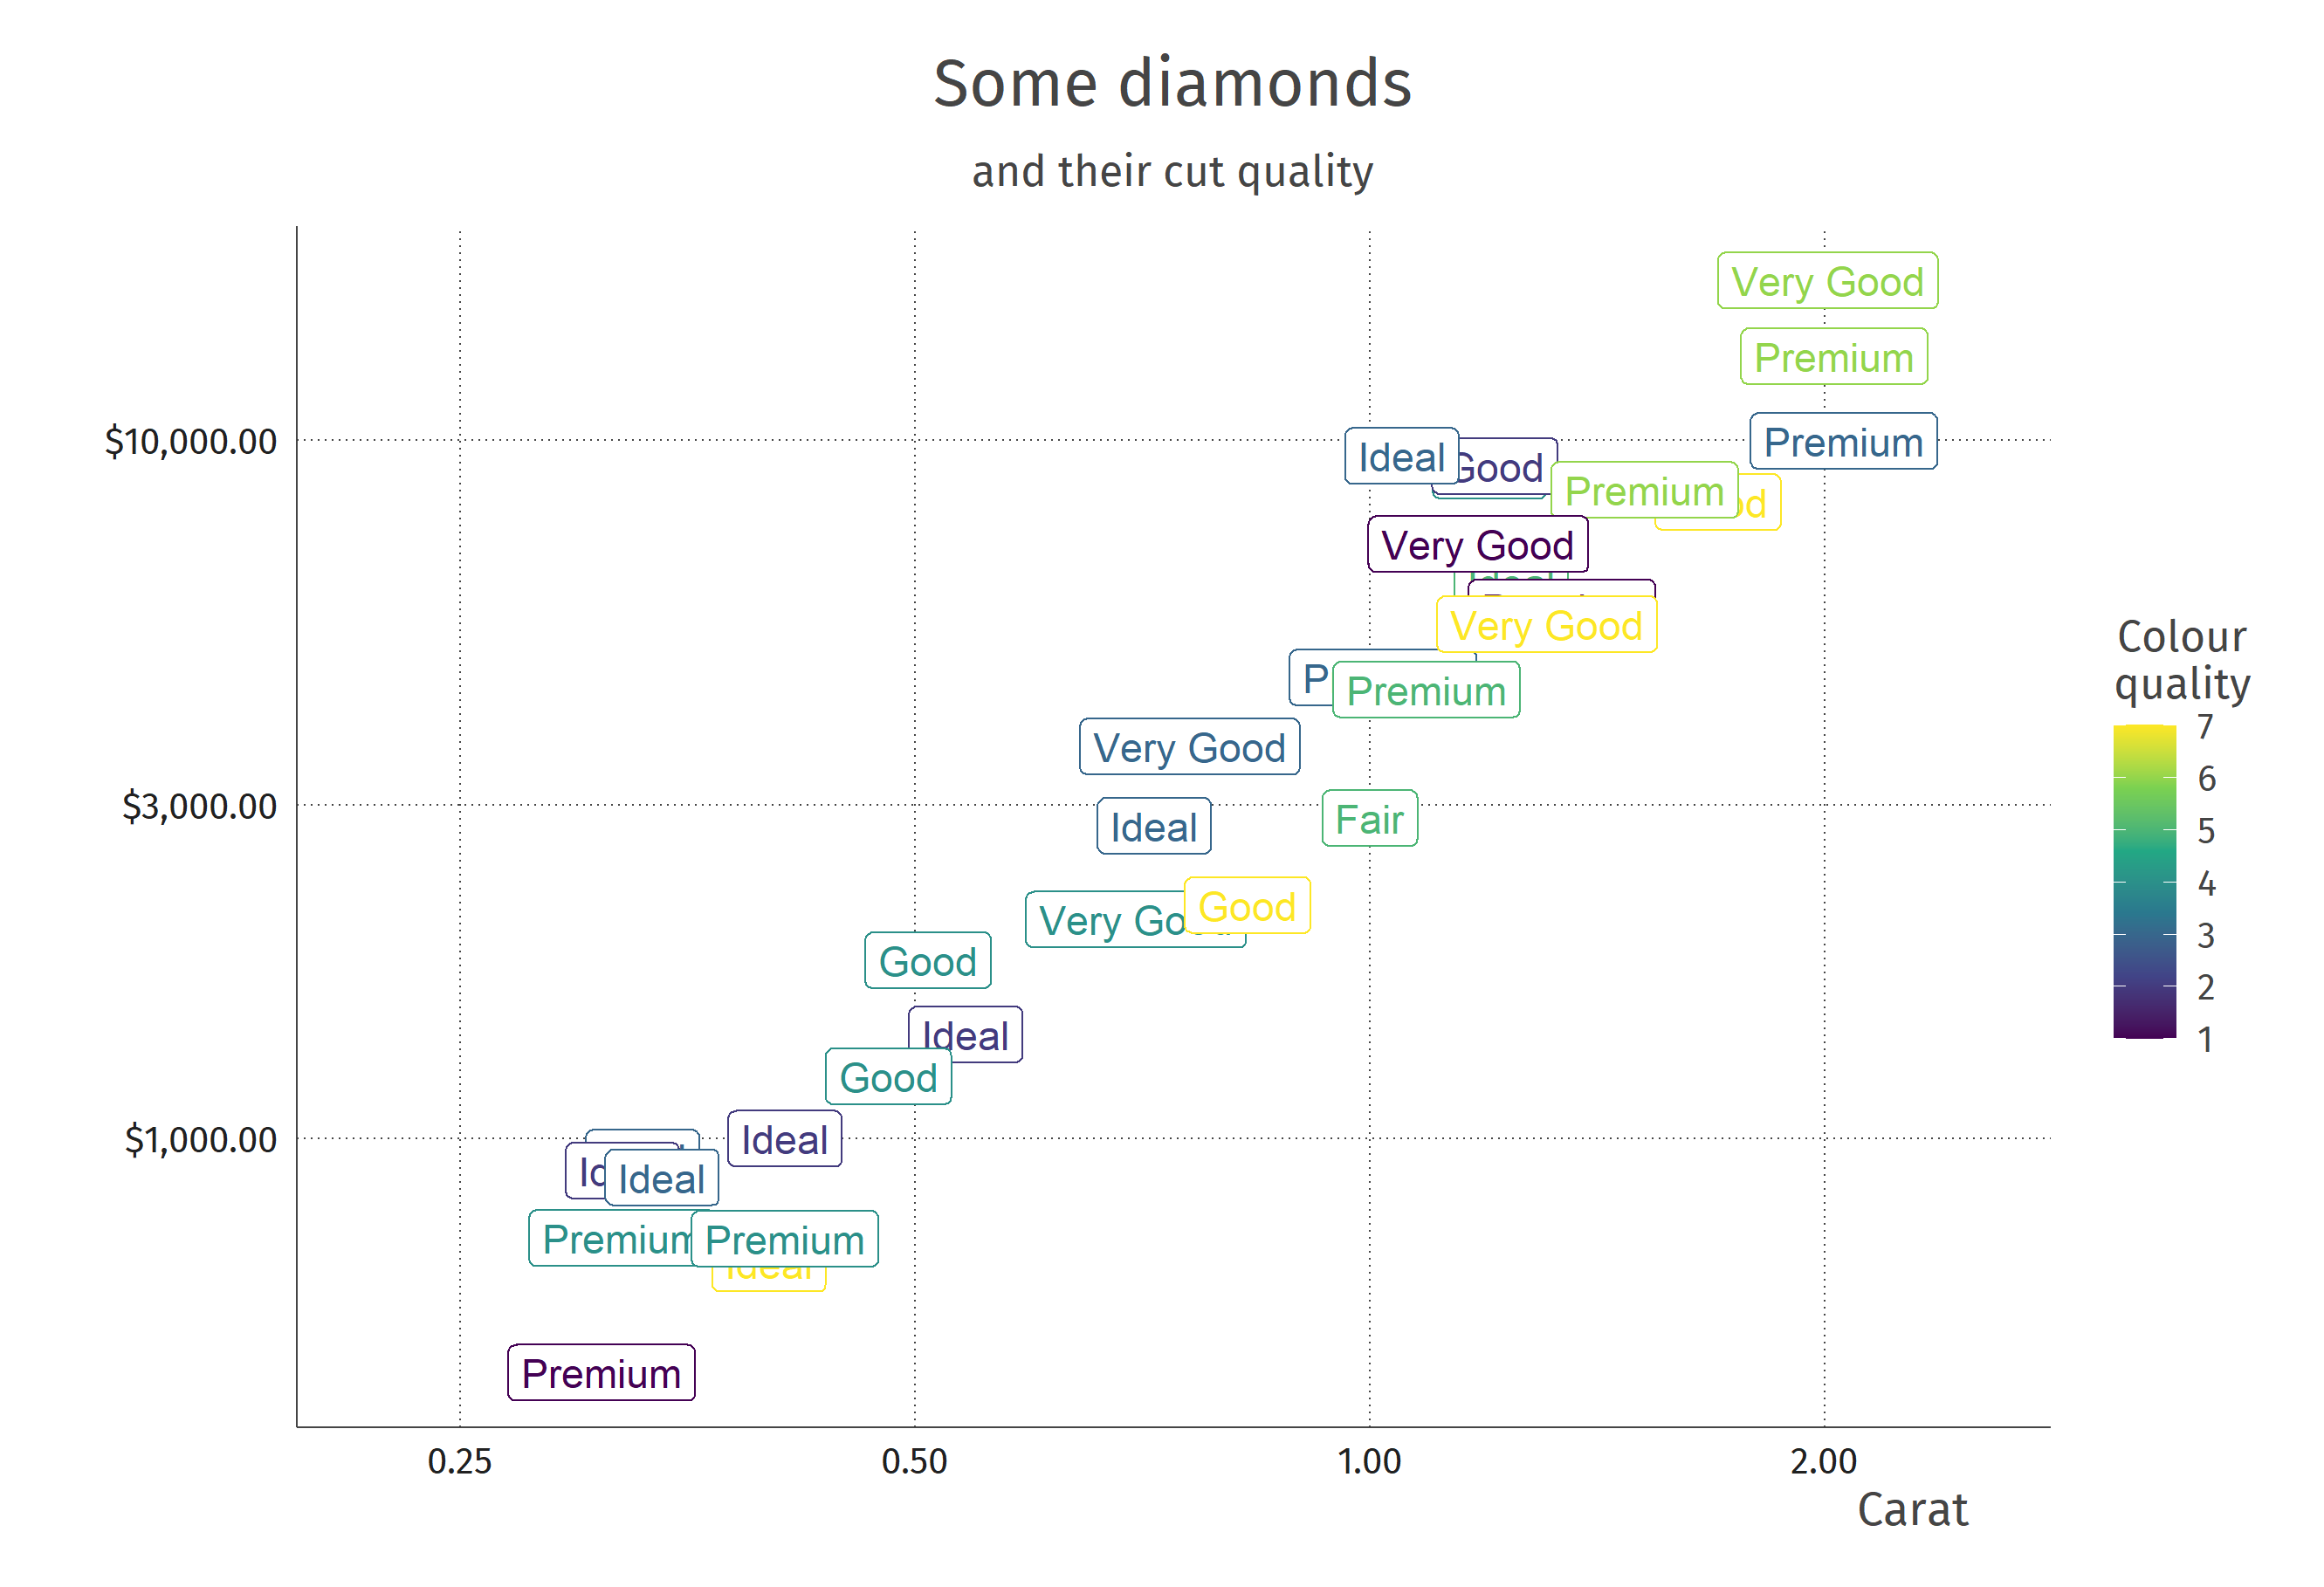
\includegraphics[width=0.78\textwidth]{pics/ggdiamonds.png}
\end{frame}

\section{Conclusion}


\begin{frame}


  Conclusion  
\end{frame}

\begin{frame}{Conclusion}

  \begin{itemize}
    \item Data visualization is a huge field;
    \item Sticking to \textbf{basic principles} helps:
      \begin{itemize}
      \item \textbf{Map data} to aesthetics, geoms, scales, facets;
    \item \text{Perception} research  guides choices;
      \item \textbf{Which comparisons} do I want?
          \item Maximize \textbf{data-ink} (within reason).
          \end{itemize}
  \end{itemize}
\end{frame}

\end{document}






